\documentclass[border=5pt]{standalone}
\usepackage{tikz}
\usetikzlibrary{arrows.meta,positioning,calc}
\usepackage{helvet}
\renewcommand{\familydefault}{\sfdefault}
\newcommand{\sys}{ActPlane}

\begin{document}
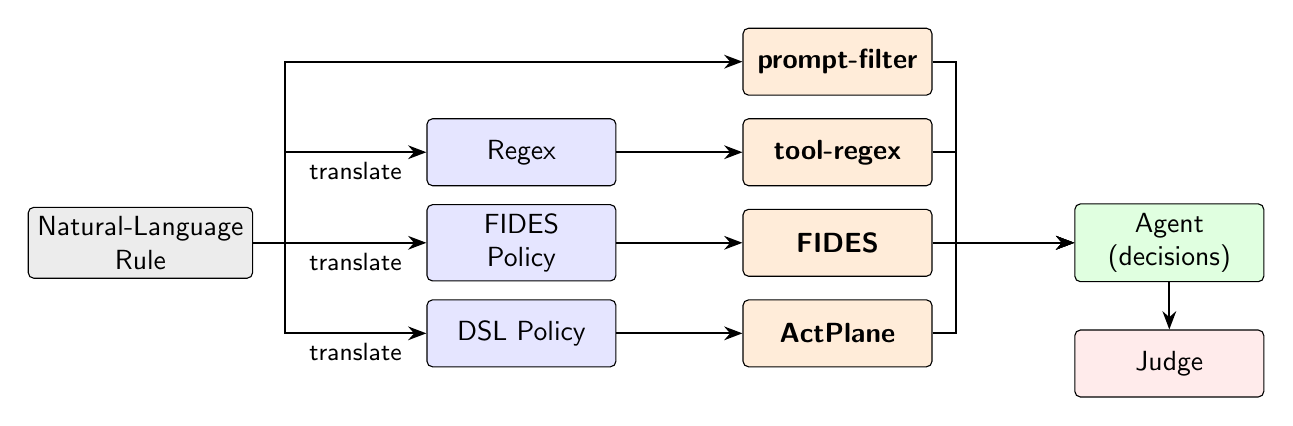
\begin{tikzpicture}[
  >=Stealth,
  box/.style={draw, rounded corners=2pt, minimum height=0.85cm,
              minimum width=2.4cm, align=center, font=\normalsize},
  arr/.style={->, thick},
]

% Start
\node[box, fill=gray!15, minimum width=2.8cm] (nl) {Natural-Language\\Rule};

% Artifacts (middle column)
\node[box, fill=blue!10, right=2.2cm of nl, yshift=1.15cm] (regex) {Regex};
\node[box, fill=blue!10, right=2.2cm of nl] (fidespol) {FIDES\\Policy};
\node[box, fill=blue!10, right=2.2cm of nl, yshift=-1.15cm] (dsl) {DSL Policy};

% Enforcement (right column) — system names as labels
\node[box, fill=orange!15, right=1.6cm of regex, yshift=1.15cm, font=\normalsize\bfseries] (e1) {prompt-filter};
\node[box, fill=orange!15, right=1.6cm of regex, font=\normalsize\bfseries] (e2) {tool-regex};
\node[box, fill=orange!15, right=1.6cm of fidespol, font=\normalsize\bfseries] (e3) {FIDES};
\node[box, fill=orange!15, right=1.6cm of dsl, font=\normalsize\bfseries] (e4) {\sys{}};

% Agent + Judge
\node[box, fill=green!12, minimum width=2.4cm, right=1.8cm of e3] (agent) {Agent\\(decisions)};
\node[box, fill=red!8, below=0.6cm of agent] (judge) {Judge};

% NL → prompt-filter (direct, no artifact)
\draw[arr] (nl.east) -- ++(0.4,0) |- (e1.west);

% NL → artifacts (via translate)
\draw[arr] (nl.east) -- ++(0.4,0) |- node[below, font=\small, pos=0.75] {translate} (regex.west);
\draw[arr] (nl.east) -- ++(0.4,0) |- node[below, font=\small, pos=0.75] {translate} (fidespol.west);
\draw[arr] (nl.east) -- ++(0.4,0) |- node[below, font=\small, pos=0.75] {translate} (dsl.west);

% artifacts → enforcement
\draw[arr] (regex) -- (e2);
\draw[arr] (fidespol) -- (e3);
\draw[arr] (dsl) -- (e4);

% enforcement → agent
\draw[arr] (e1.east) -- ++(0.3,0) |- (agent);
\draw[arr] (e2.east) -- ++(0.3,0) |- (agent);
\draw[arr] (e3.east) -- ++(0.3,0) |- (agent);
\draw[arr] (e4.east) -- ++(0.3,0) |- (agent);

% agent → judge
\draw[arr] (agent) -- (judge);

\end{tikzpicture}
\end{document}
